\documentclass[12pt]{report}
\usepackage[utf8]{inputenc}
\usepackage[T1]{fontenc}
\usepackage[francais]{babel}
\usepackage{graphicx}
\usepackage{amsfonts}
\usepackage{hyperref}

\usepackage{array}
\usepackage{titlesec}
\usepackage{amssymb}
\usepackage{diagbox}
\usepackage{geometry}
\geometry{hmargin=2.5cm,vmargin=1.5cm}

\titlespacing*{\subsection}{30pt}{15pt}{10pt}
\titlespacing*{\subsubsection}{0pt}{15pt}{5pt}

% Packages graphiques
\usepackage{caption} 
\usepackage{tikz}
\usepackage{mathtools}
\usepackage{amsmath}
\usepackage{pgfplots}
\usepackage{pdfpages}
\usetikzlibrary{plotmarks}
\pgfplotsset{compat=1.8}

\renewcommand{\thesubsubsection}{}
\renewcommand{\theparagraph}{}
\usepackage{blindtext}
\usepackage{chngcntr}
\counterwithin*{section}{chapter}

\title{Guidage d'un personne malvoyante via une application GPS sur smartphone}
\author{Guitard \and Ouaraqua Dantchiawa \and Marcy \and Berthelot}
\date{\today}
\begin{document}
\setcounter{secnumdepth}{3}
\begin{titlepage}

\newcommand{\HRule}{\rule{\linewidth}{0.5mm}} 


\center 
 


\textsc{\LARGE Université de Bordeaux}\\[1.5cm] 
\textsc{\Large Département Informatique}\\[0.5cm] 
\textsc{\large Projet de Programmation}\\[0.5cm] 

%----------------------------------------------------------------------------------------
%	TITRE
%----------------------------------------------------------------------------------------

\HRule \\[0.5cm]
{ \LARGE \bfseries Guidage d’une personne malvoyante via une application GPS sur smartphone}\\[0.5cm]
\HRule \\[1.5cm]
 
%----------------------------------------------------------------------------------------
%	AUTEURS
%----------------------------------------------------------------------------------------

\begin{minipage}{0.4\textwidth}
\begin{flushleft} \large
\emph{Auteurs:}\\
Alan \textsc{Guitard}\\
Mohamed \textsc{Ouaraqua Dantchiawa}\\
Nicolas \textsc{Marcy}\\
Florian \textsc{Berthelot}\\

\end{flushleft}
\end{minipage}
~
\begin{minipage}{0.4\textwidth}
\begin{flushright} \large
\emph{Encadrant:} \\
Matthieu \textsc{Raffinot}\\
\emph{Client:}\\
Serge \textsc{Chaumette} 
\end{flushright}
\end{minipage}\\[2cm]



%----------------------------------------------------------------------------------------
%	DATE 
%----------------------------------------------------------------------------------------

{\large \today}\\[1.5cm] % Date

%----------------------------------------------------------------------------------------
%	LOGO
%----------------------------------------------------------------------------------------


\includegraphics[height=80px]{bxlogo.jpg}\\[1cm] % Logo université
 
%----------------------------------------------------------------------------------------

\vfill 

\end{titlepage}



\tableofcontents

\newpage

\chapter*{Introduction}
\addcontentsline{toc}{chapter}{Introduction}
\setcounter{chapter}{1}

L'application demandée est une application \textit{Android} utilisant le GPS fourni par l'outil \textit{Google Maps}, afin de guider une personne malvoyante sur un trajet de piéton. Elle aura pour but de fournir à l'utilisateur un moyen de se guider dans une ville par ses propres moyens. On proposera un moyen de synchroniser deux téléphones pour pouvoir indiquer facilement la route à suivre. \\
Par demande du client, une version 1.0 sera proposé en tant que prototype. Il est à noter que l'utilisation de cette application ne remplace pas les moyens habituelles de l'utilisateur qu'il utilise pour se déplacer seul (canne, chien d'aveugle,...). L'application n'est responsable d'aucun accident physique, l'utilisateur est seul responsable.

\chapter*{Besoins non-fonctionnels}
\addcontentsline{toc}{chapter}{Besoins non-fonctionnels}

\section{Interface}

\subsection{Description}
\`A l'ouverture de l'application, il y sera affiché simplement une invitation de saisie de texte pour entrer une destination et un bouton mégaphone. L'API est à tester pour savoir à quel point la recherche vocale d'un lieu est précise. Il est quand même offert la possibilité d'écrire du texte, permettant à une tiers personne d'entrer l'adresse de la destination manuellement. Ici, le vibreur ne sera pas utile.\newline 

\begin{figure}[ht]
\begin{center}
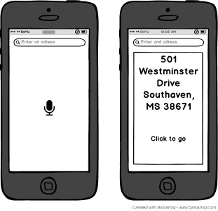
\includegraphics[]{first.png}
\caption{Interface de saisie d'adresse}
\end{center}
\end{figure}

Quand une adresse est validée, elle est sauvegardée dans la mémoire du téléphone. Les écrans en figure 2.1 sont interchangeables par simple mouvement du doigt vers la droite ou vers la gauche pour parcourir la liste de patrons suivants : Bouton de saisie vocale et textuelle -> adresse 1 -> adresse 2 -> ...\newpage -> adresse n. \emph{Une version avancée du prototype aura un menu Paramètres qui proposera à l'utilisateur de définir son protocole de priorités d'application (Voir Problèmes envisagés)}.

\subsection{Contraintes}

\subsubsection{Ergonomie}
L'interface se doit d'être le plus ergonomique possible afin de permettre à un utilisateur non-voyant de naviguer dans les menus avec le plus de facilité possible. Chaque item du menu fera l'objet d'une activité qui prendra tout l'écran, il pourra aussi être envisagé de faire dicter par une boite vocale ce qu'il y a écrit. A chaque changement d'activité, le téléphone vibrera afin de signifier le changement d'activité.

\subsubsection{Robustesse et stabilité}
L'ensemble des activités doit être accessibles à partir des autres activités, un test doit donc être réalisé sur le graphe des activités pour vérifier qu'il est fortement connexe. Pour tester que l'application ne s'éteint pas prématurément à cause d'un bugs, un oracle doit être implémenté. Cet oracle devra aléatoirement se déplaçait dans les activités afin d'augmenter la confiance en la robustesse et la stabilité de l'application.

\section{Synchronisation} 

\subsection{Description}
Une fois que l'utilisateur valide une adresse, l'application cherchera les appareils BlueTooth visibles. 
Les deux téléphones doivent avoir chacun l'application installée, mais les deux n'auront pas le même comportement. L'un sera serveur et l'autre client. Celui qui cherchera sera considéré comme le serveur et, par convention pour commencer, il sera celui qui sera assigné à la vibration droite. Le serveur sera celui qui recevra les données de Google Maps, qui fera les calculs et qui enverra les signaux aux clients pour le faire vibrer

\subsection{Contraintes}

\subsubsection{Ergonomie} Pour se synchroniser avec un autre appareil, il faut trouver un moyen efficace et simple qui fournit à un aveugle la possibilité de se connecter en BlueTooth sans boîte vocale. Si cela est possible (les possibilités du SDK d'Android sont à vérifié), une liste similaire à la liste des adresses devra être implémentée (Voir Interface en 2.1). Cette liste fera figure de sur-couche de la boite de dialogue d'Android, permettant à l'utilisateur de choisir avec plus d'ergonomie l'appareil cible. Lorsqu'il aura choisi, l'appareil cible se fera reconnaître de l'utilisateur par une vibration à la demande d'appareillage, de sorte à indiquer à l'utilisateur qu'il doit maintenant appuyer sur l'écran des deux téléphones afin de valider la synchronisation.

\subsubsection{Performance} Ils doivent pouvoir recevoir des ondes ou les émettre et ce, d'une rapidité convenable pour simuler un temps réel (estimé à moins d'une seconde de latence).

\subsubsection{Batterie}
Lorsque la batterie de l'un des deux téléphones se décharge, l'application ne sera plus en mesure de pouvoir guider l'utilisateur puisque la synchronisation sera arrêtée. La vibration sera utilisée pendant trois secondes sur le téléphone non déchargé pour indiquer à l'utilisateur que la synchronisation s'est arrêtée. L'application relancera automatiquement une nouvelle tentative de synchronisation. \emph{La recherche des appareils BlueTooth visibles est coûteuse en énergie, elle est à faire le moins possible.}

\subsubsection{Sécurité}

Du point de vue sécurité, l'application serveur doit empêcher l'utilisateur mal-voyant de se connecter par mégarde à un appareil tiers. Une confirmation doit donc être envoyé par le client. Également, l'application client ne doit pas laisser un appareil tiers se connecter à lui. 
Les développeurs ne sont pas responsables des accidents qui surviendraient de l'utilisation de l'application sur des téléphones défectueux ou obsolètes qui créeraient des désynchronisations.

\section{Guidage}

\subsection{Description}

\begin{figure}[ht]
\begin{center}
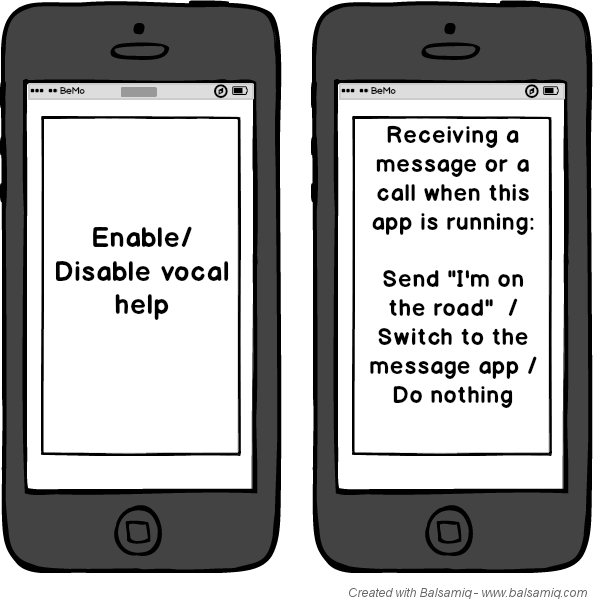
\includegraphics[scale=0.3]{Mobile_example.png}
\caption{Interface durant le guidage}
\end{center}
\end{figure}

L'application doit pouvoir guider un utilisateur sans que ce dernier n'ait à regarder sur la carte. Il sera potentiellement dans deux états lorsqu'il sera en route: un état où il devra marcher tout droit jusqu'à la prochaine intersection (qu'on nommera ici \textit{Straight}), et un état où il sera à une intersection (qu'on nommera \textit{Cross}). Plusieurs hypothèses de travail sont envisagées:
\paragraph{État \textit{Straight}: } L'application avertira par une vibration saccadée qu'un mauvais chemin a été pris, et qu'il doit faire demi-tour. Au bout de 2 avertissements, un nouvel itinéraire qui permettra au malvoyant de retrouver son chemin sera recalculé. Pour signaler l'arrivée à la destination finale, le téléphone vibrera d'une vibration continue.
\paragraph{État \textit{Cross}: } Grâce aux deux portables synchronisés par BlueTooth, le code devient simple pour indiquer la route à suivre. Un téléphone sera délégué de vibrer pour dire à l'utilisateur d'aller à gauche, et l'autre téléphone à droite.

\subsection{Contraintes}
\subsubsection{Performances} L'application ne doit pas afficher une localisation qui date de plus d'une seconde en mémoire, afin que le guidage soit le plus fluide possible. Les tests de performances doivent vérifier que, en moins d'une seconde, le téléphone principal reçoit les données de position et les envoie au téléphone secondaire en moins d'une seconde.

\subsubsection{Capacité} L'application a un besoin constant de connexion internet et d'une bande passante convenable qui satisfait les besoins en performance. Ces contraintes sont les mêmes en ce qui concerne la connexion BlueTooth.

\subsubsection{Disponibilité}
Afin de pouvoir utiliser l'application il est nécessaire d'avoir une connexion internet, elle est utilisable seulement dans un lieu où le téléphone est susceptible de recevoir les données nécessaires au bon fonctionnement de celle-ci. De plus l'application ne marchera uniquement dans les lieux qui sont couverts par l'API cartographique de Google.

\subsubsection{Stabilité du code} Des tests doivent être fournis qui permettront de certifier la bonne validité du code. 
\subparagraph{Tester les itinéraires} Le module de calcul d'itinéraire doit faire faire l'objet de tests de régression afin de certifier ses résultats.
\subparagraph{Tester les fonctions vibreur} L'application cliente doit vibrer \emph{si et seulement si} l'application serveur est à une intersection et l'itinéraire (certifié) indique la gauche ou que l'utilisateur est en sens inverse. Les mêmes tests sont requis pour l'application serveur. Quand un mauvais chemin est emprunté, les deux applications vibrent de concert un court temps avant de recalculer un itinéraire.

\subsubsection{Problèmes envisagés}
\subparagraph{} Pour le code à établir pour le vibreur, un simple code pour gauche ou droite ne suffira pas, car une intersection peut avoir plus de 4 routes qui s'y rattache. Dans le cadre d'un premier prototype, et par concertation avec le client, cette éventualité sera ignorée afin de permettre en premier lieu un guidage par intersection simple.
\subparagraph{} L'application utilisant le vibreur constamment, il faut convenir d'un protocole lorsque le téléphone reçoit un appel, un message, une notification. En d'autres termes, il ne faut pas que le code vibreur soit faussé par une autre application. Là aussi, il est demandé par le client que le premier prototype ne s'occupera pas de ces possibles conflits. 

\subsubsection{Sécurité}
Pour un fonctionnement optimal de l'application, l'utilisateur doit donc désactiver toute autre application pouvant utiliser le vibreur. Dans le cas contraire, l'utilisateur s'expose à des conflits qui pourrait mener à des mauvaises indications de direction, et il en sera le seul responsable. \emph{ A titre informatif: Deux choix de conception sont possibles: imposer un protocole ou en laisser l'utilisateur le choix en proposant dans les paramètres un menu l'invitant à définir le comportement de l'application pour chaque événement.}

\section{Documentation}
Une documentation du code source sera fourni afin de rendre l'application plus maintenable. Tous les membres du projet devront suivre des règles de codage communes afin de rendre le code source final lisse et homogène.

\newpage
\chapter*{Besoins fonctionnels}
\addcontentsline{toc}{chapter}{Besoins fonctionnels}
\setcounter{chapter}{2}
\setcounter{section}{0}
\label{ch:BF}

\section{Environnement de programmation}

\subsection{Choix de l'IDE} Après quelques tests effectués avec Android Studio et Eclipse (couplé au plugin ADT -Android Development Tools-), les deux semblent convenir pour un bon développement. Eclipse sera moins lourd à supporter pour certaines machines, mais Android Studio dispose d'un meilleur suivi de Google. Tant que tout les autres contraintes sur le dépôt principal du projet, ce choix appartient au développeur\footnote{\url{http://www.android-dev.fr/presentation_de_android_studio_et_comparatif_avec_adt\#.VqtxiWfR9mM}}.

\subsection{Android SDK 4.4 Kit-Kat } L'application sera codé en Java, couplé par le XML que nous propose l'architecture d'Android. La version 4.4 du kit de développement d'Android KITKAT sera utilisée, afin que l'application fonctionne sur le plus d'appareils possible. Malgré tout, la version qui sera utilisé pourra en être une autre, mais toujours en préconisant la visibilité de l'application.

\subsection{Gestionnaire de versions } Un gestionnaire de versions va être utilisé afin de disposer d'un dépôt local commun au projet, et d'avoir la possibilité de récupérer des versions ultérieures en cas d'erreur locale. Tout au long du projet, Git sera utilisé de permettre aux membres du projet de travailler sans internet, étant un gestionnaire de versions décentralisé. Savane sera utilisé en tant que dépôt de release intermédiaire et final.

\subsection{Google Maps API } 
\paragraph{Algorithme d'itinéraire} L'interface de Google Maps Directions sera testée. Cette dernière renvoie une suite de maximum 23 points (limite standard) constituant l'itinéraire calculé. Pendant le développement, cette API pourrait se révéler trop peu précise pour les besoins de l'application. Du temps devra alors être consacré à l'extension ou à la création d'un nouvel algorithme plus adapté. 
\paragraph{Algorithme de géolocalisation} La géolocalisation a quant à elle une limite standard de 10 requêtes par seconde par utilisateur, dans une limite de 2500 par jour.

\subsection{Matériels } Les émulateurs d'appareils Android étant très lent, le client s'engage à fournir des équipements de tests, en l'occurrence des téléphones fonctionnant sous Android, afin de travailler dans les meilleurs conditions.\\

\subsection{Tests avec JUnit4 }
Afin de réaliser les tests de nos fonctionnalités et de nos codes, Android SDK fournit un module de test se nommant JUnit\footnote{\url{http://developer.android.com/tools/testing/testing_android.html}}, la version 4 sera utilisé pour profiter au mieux du progrès de développement de JUnit. 
\paragraph{Tests de régression:} Tout les tests  seront utilisés au long du projet afin de vérifier que les nouvelles fonctionnalités apportées ne dérangent pas le bon fonctionnement des précédentes.

\section{Gestion de la mémoire, SQLite} La librairie SQLite sera utilisée pour:
\begin{itemize}
\item Sauvegarder sur la mémoire du téléphone les adresses que l'utilisateur veut enregistrer. 
\item Sauvegarder régulièrement le reste du trajet à effectuer en cas de crash de l'application et/ou de fermeture impromptue. 
\end{itemize} Pour ce dernier point, le SDK d'Android fournit une fonction de Backup\footnote{\url{http://developer.android.com/guide/topics/data/backup.html}} qui sera probablement préférable à SQLite, en termes de coût de développement.\\

Il a été choisi SQLite car c'est un système de gestion de base de données déjà intégré au SDK d'Android et qu'elle est accessible par le langage SQL. SQLite a une portabilité assez facile ce qui pourra permettre une extension de l'application sur d'autres systèmes. Étant un libraire libre qui appartient au domaine public, aucune licence n'est requise pour l'utiliser. 

   \section{Synchronisation} Pour la synchronisation entre deux téléphones, le kit de développement fournit des fonctions afin d'interagir par BlueTooth avec un appareil distant. Les deux appareils doivent donc avoir chacun l'application d'installée. 

\textbf{Protocole de discussion BlueTooth:} Il faut donc convenir d'un protocole de discussion, à l'instar de TCP ou UDP, adapté au BlueTooth. Vu que les deux téléphones auront l'application, le téléphone qui a fait la demande de synchronisation sera utilisé comme serveur et délégué à la vibration droite. Le deuxième téléphone sera le client et vibrera pour indiquer de tourner à gauche. L'appareil client ne calculera pas les itinéraires, il sera juste chargé de vibrer lorsque l'appareil serveur lui signalera tandis que ce dernier calculera l'itinéraire et l'affichera en plus de son rôle de serveur.

\section{Documentation}
Afin de créer une documentation complète de l'application, l'utilisation de Javadoc sera nécessaire car notre application sera développée en langage Java. Javadoc a été choisi car l'ensemble des membres du groupe y est habitué.\\
L'anglais sera utilisé pour tout ce qui est linguistique (nom de variables, commentaires,...). En ce qui concerne la sémantique:
\begin{itemize}
\item \textbf{Noms de classes: } Commence par une majuscule et le reste en minuscules ou chiffres.
\item \textbf{Noms de variables: } Tout en minuscules ou chiffres.
\item \textbf{Variables, classes, fonctions ou méthodes à plusieurs mots: } Chaque début de mot (sans compter la première lettre du nom qui a déjà sa convention) doit être en majuscule. Exemple: nomDeVariable, NomDeClasse, doIt(),getMember().
\item \textbf{Compréhension: } Les noms de variables doivent avoir du sens et ne doivent pas être des termes génériques comme par exemple variable1 ou variable2.
\item \textbf{Commentaires: } Chaque fonction et classe doit être commentée par la convention initialement établie par la JavaDoc. 
\item \textbf{Mise à jour: } Quand un test est réalisé et qu'une fonction, classe, méthode ou activité est déclarée certifié par les tests, une date de validation permettra de savoir quand a été fait le dernier test. La comparaison avec la date de dernière modification sur le gestionnaire de versions permettra de savoir si le changement doit être couplé d'un nouveau test, afin de mettre à jour la validité du code.
\end{itemize}

\newpage
\chapter*{Besoins organisationnels}
\addcontentsline{toc}{chapter}{Besoins organisationnels}
\setcounter{chapter}{3}
\setcounter{section}{0}

\section{Diagramme de Gantt}

\begin{flushleft}
\begin{tabular}{|l|c|c|c||c|c|c|c|c|c|c||c|}
  \hline
  \diagbox{Tâches}{Semaine} & 5 & 6 & 7 & 8 & 9 & 10 & 11 & 12 & 13 & 14 & 15 \\
  \hline
  Téléchargement des cartes & X & & & & & & & & & & \\
  Géolocalisation & X & X & & & & & & & & & \\
  Calcul d'itinéraires & & X & & X & X & X & & & & & \\
  Mise en place de l'interface & & X & & X & X & X & X & X & & & \\
  Tests de guidage basique & & & X & & & & X & & & X & X \\
  Synchronisation BlueTooth & & & & X & X & X & & & & & \\
  Mise en place du protocole client/serveur & & & & X & X & X & & & & & \\
  Liaison vibreur / Application & & & & & X & X & X & & & & \\
  Persistance des données & & & & & & & & X & X & & \\
  Tests de guidage avancée & & & & & & & & X & X & X & X \\
  \hline
\end{tabular}
\end{flushleft}
\begin{itemize}
\item Semaine 7 (mercredi 17 Février): Rendu de la première release du code.
\item Semaine 14 (mercredi 6 avril): Mémoire et release finale du code.
\end{itemize}

\newpage
\section{Diagramme de flux de données}

\begin{figure}[ht]
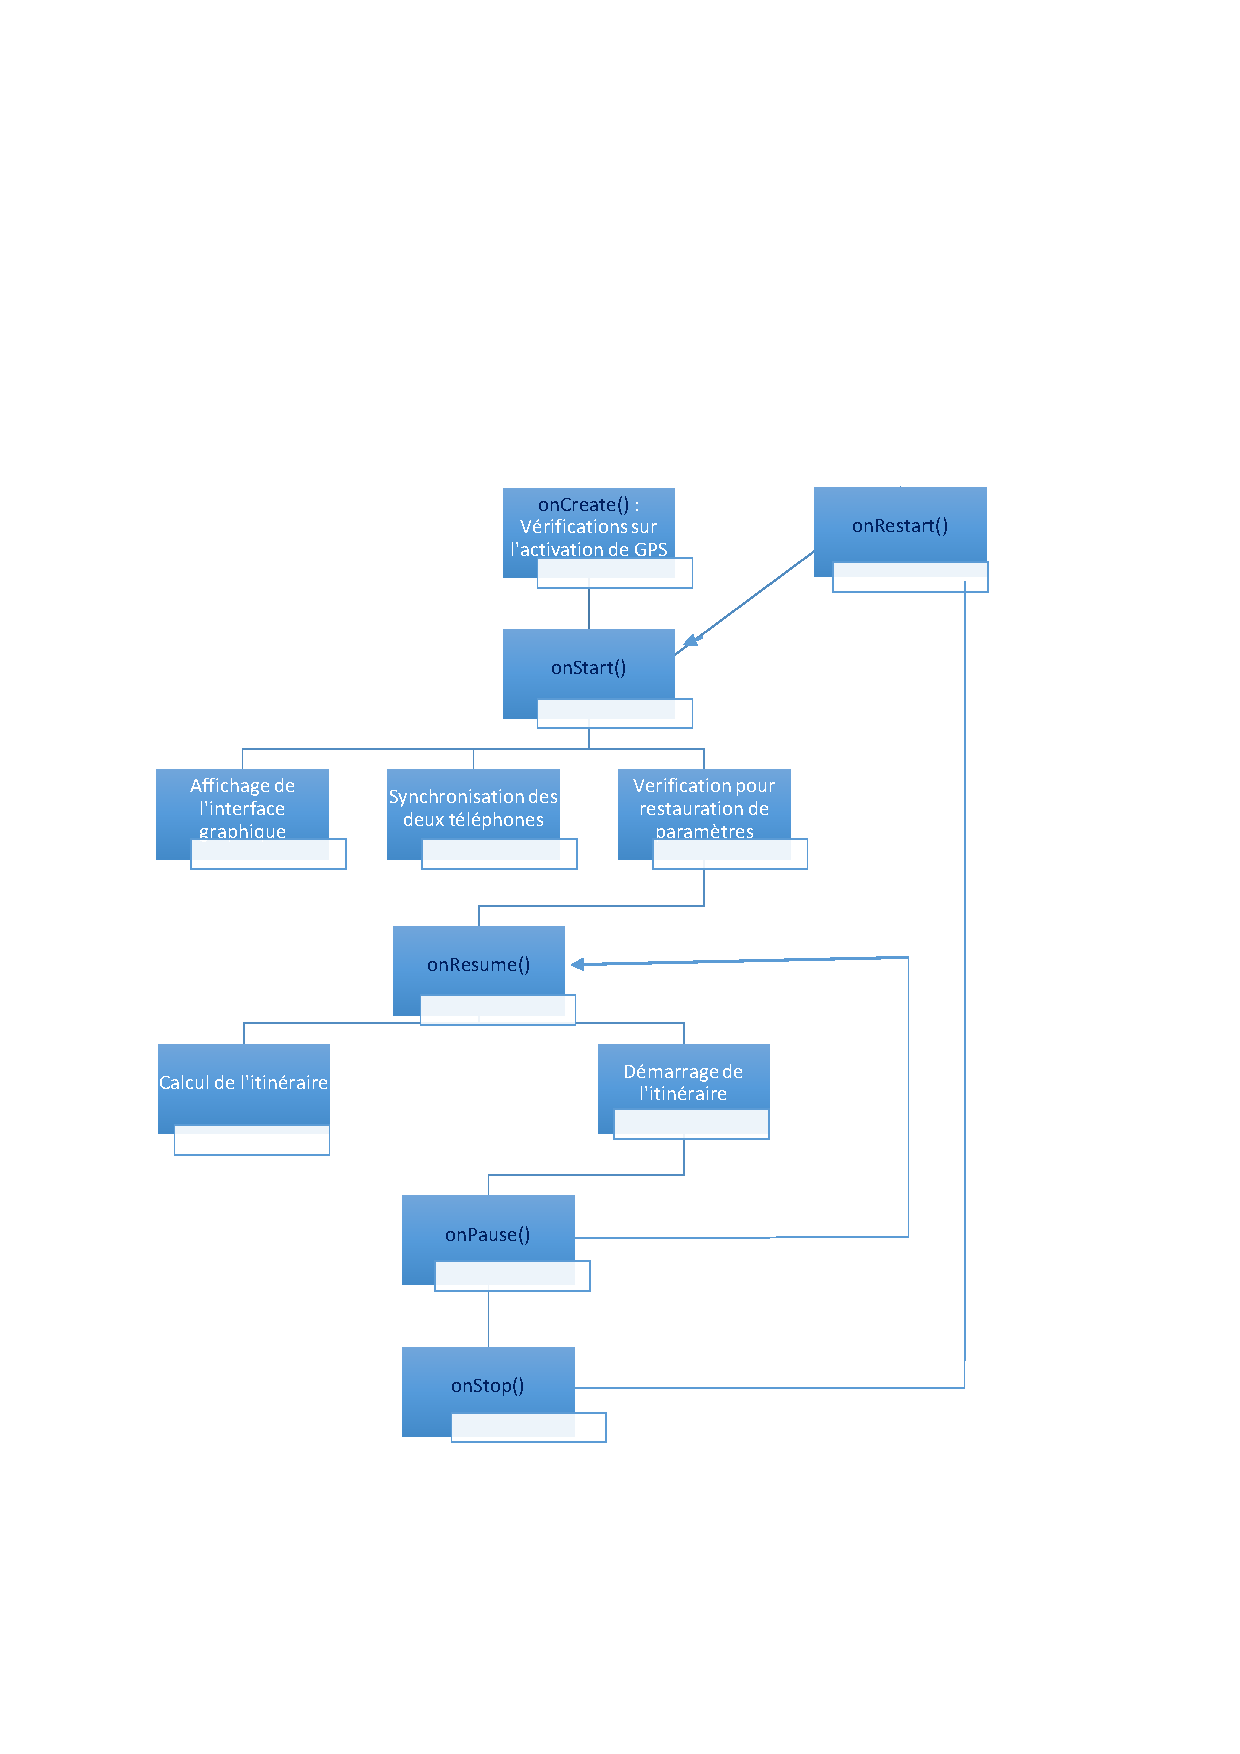
\includepdf[pages=-]{diagramme.pdf}
\end{figure}
\newpage

\section{Scénarios envisagés}

\begin{figure}
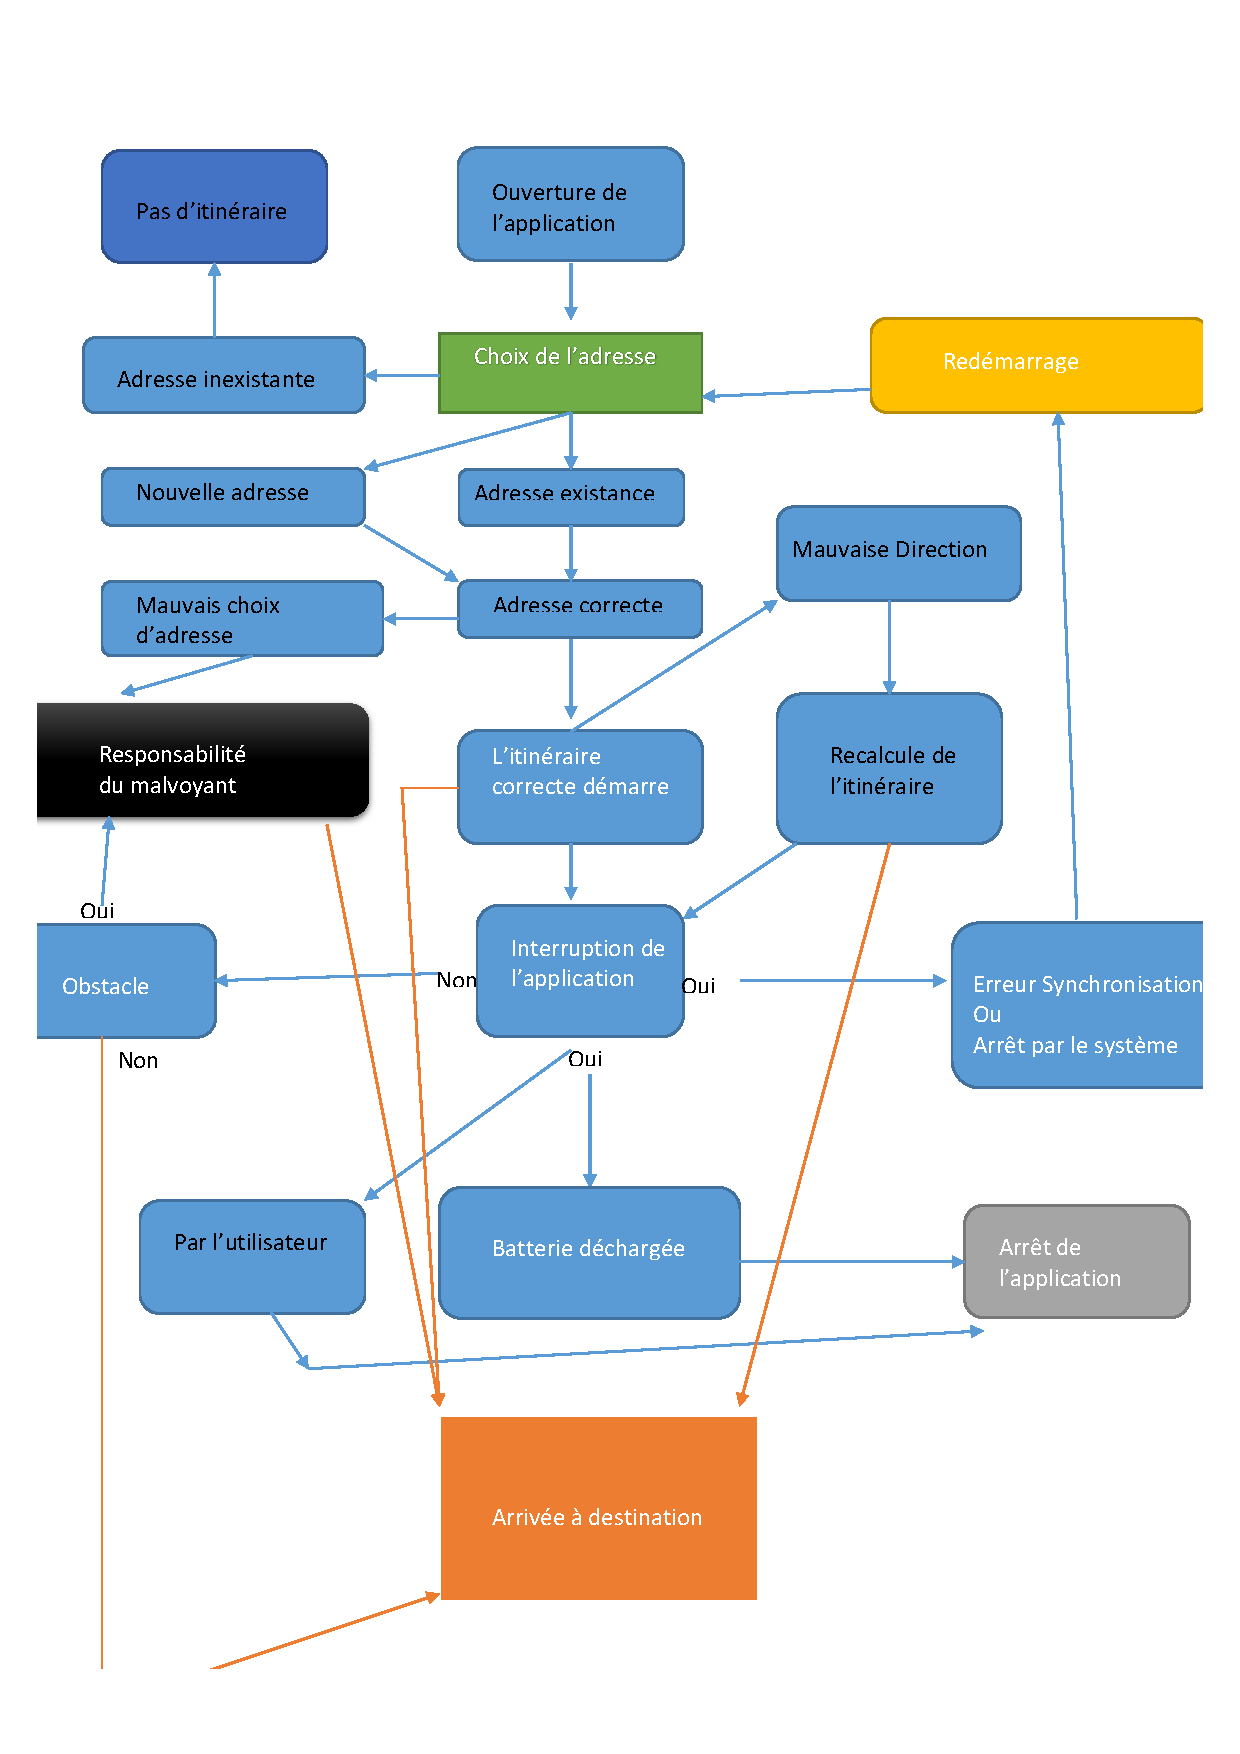
\includepdf[scale=0.8]{scenario__2_.pdf}
\end{figure}

\newpage
L'image ci-dessous montre le cas où l'utilisateur se rapproche d'une intersection où il devra tourner à gauche. Le smartphone de droite "serveur" qui possède la carte avec l'itinéraire devra donc signaler au smartphone de gauche de vibrer.\\\\
\begin{figure}[h]
\begin{center}
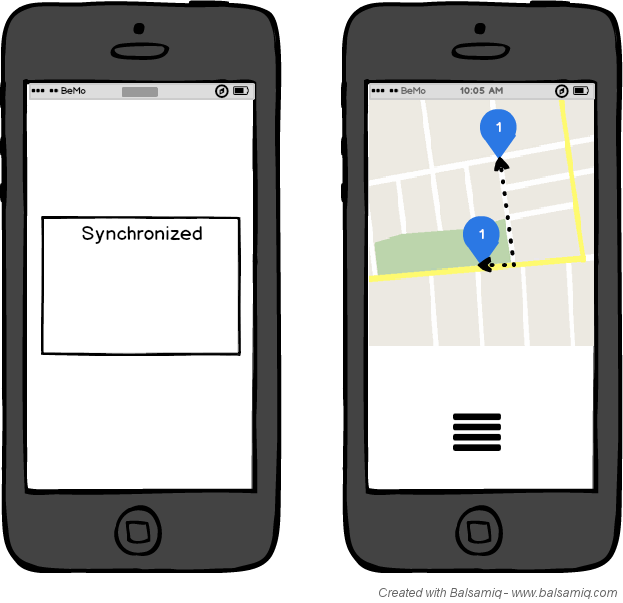
\includegraphics[scale=0.5]{Cas.png}
\caption{Synchronisation}
\end{center}
\end{figure}

\chapter*{Bibliographie}
\begin{itemize}
\item SQLite: \url{https://www.sqlite.org/about.html}
\item Google Maps API:\\ \url{https://developers.google.com/maps/documentation/android-api/?hl=fr}
\item Android SDK: \url{http://developer.android.com/develop/index.html}
\item Apache Subversion: \url{https://subversion.apache.org/}
\item GitHub: \url{https://github.com/}
\item JavaDoc: \url{http://www.oracle.com/technetwork/articles/java/index-jsp-135444.html}
\item Eclipse: \url{https://eclipse.org/}
\end{itemize}
\end{document}
